In questo capitolo verrà discusso dell'algoritmo C.U.T.E e
del contributo apportato da questo nuovo approccio nell'ambito del \textit{clustering} dei dati di traiettoria.

In primo luogo verrà definito il problema del \textit{Colossal Trajectory Mining},
successivamente saranno presentate l'idea e la realizzazione dell'algoritmo C.U.T.E,
infine saranno formulate alcune considerazione sui punti di forza e limiti di questo nuovo approccio.


\section{Colossal Itemset Mining}\label{sec:cute:cim}
Negli ultimi anni, la maggiore disponibilità di risorse, le nuove tecniche di elaborazione dati e piattaforme Big Data ha reso possibile gestire dataset di dimensioni sempre maggiori.
A crescere però non è solo il numero dei dati, ma anche la loro dimensionalità.
Un caso su tutti è l'ambito bio-informatico: i dataset di espressione dei geni raggiungono 10.000-100.000 attributi per 100-1000 righe.
Questi dataset sono una sfida per le tecniche di frequent itemset mining per la seguente ragione:
il numero di itemset candidati cresce esponenzialmente rispetto alle dimensioni del set di attributi.
Ciò implica che con elevati numeri di attributi, la generazione con le tecniche classiche, come Apriori \cite{agarwal2001tree}, diventi proibitiva.
Conseguentemente al numero dei candidati aumenta esponenzialmente anche il numero degli itemset frequenti.
Sono generati infatti, per ogni set frequenti, tutti i suoi possibili subset, in quanto loro stessi frequenti.

Il \textit{colossal itemset mining} si pone come un'estensione del frequent itemset mining volta ad approcciare i dataset con le caratteristiche descritte sopra.
Questa espansione riguarda l'utilizzo di dati a elevata dimensionalità~\cite{zhu2007mining} all'interno delle operazioni di mining.
Il principale cambiamento che permette al colossal itemset mining di essere efficiente nell'esplorazione dei possibili itemset sono le proprietà ricercate sopra questi ultimi.
Gli itemset prodotti sono infatti o chiusi (\cref{definition:closed-itemset}) o massimali (\cref{definition:maximal-itemset}).
Generando solo pattern di queste due categorie lo spazio di ricerca cala, sebbene non calino le dimensioni degli itemset individuati.
Affrontando la ricerca con le tecniche di mining tradizionali, come ad esempio Apriori (\cref{subsec:apriori}), il numero di itemset generati e valutati nel caso peggiore è \(2^n\), dove \(n\) è il numero di attributi del dataset.
Analogamente, dato un itemset chiuso di \(m\) elementi, le ricerche di mining tradizionali richiedono di generare quel pattern e i \(2^m\) figli frequenti per definizione di monotonicità.
Gli algoritmi di mining colossale non esplorano questi  \(2^m\) figli frequenti e mantengono solo l'itemset chiuso.
Il numero di pattern individuati e i tempi necessari calano quindi drasticamente, a scapito della granularità della ricerca.

La ricerca di questi pattern è limitativa, ma può produrre comunque risultati validi. 
Nei casi in cui il dataset abbia un numero elevato di attributi, molto spesso sono ritenuti ``interessanti' solo i gruppi di attributi particolarmente lunghi.
La ragione è che spesso questi pattern hanno un maggior significato rispetto agli itemset più corti~\cite{zhu2007mining}.
Ad esempio nell'ambito della bioinformatica sequenze genetiche più lunghe e complesse sono più indicative per determinare la predisposizione a certe malattie.
Al contrario sequenze brevi hanno spesso relazioni più deboli con potenziali problematiche.


\subsection{Estrazione di itemset colossali:Carpenter}\label{subsec:cute:carpenter}
Carpenter~\cite{pan2003carpenter} è uno dei principali framework per
la ricerca di itemset su dataset ad alta dimensionalità.

Scopo dell'algoritmo è la ricerca di itemset colossali chiusi su dati ad alta dimensionalità.
Questo algoritmo individua insiemi di feature frequenti generando una versione trasposta del dataset originale, chiamata \textit{TT}, e un albero, chiamato \textit{row enumeration tree} avente nei nodi tutti i possibili set di transazioni;
successivamente questo viene esplorato utilizzando una ricerca \textit{depth-first}.

Il punto di partenza di Carpenter consiste in un insieme di transazioni \(D\) che contiene \(F\) attributi possibili.
Su questo sono definite due funzioni: si definisce funzione di calcolo del supporto di un set di attributi \(\mathcal{R}\) la funzione che dato un insieme di attributi \(F'\) calcola il numero totale di righe che li contiene.
Si noti che \(\mathcal{R}\) è analogo alla funzione \(s\), che dato un itemset ne calcola il supporto, presentata nella \cref{sec:fim}.
Analogamente si definisce funzione di calcolo del supporto comune ad un insieme di righe \(\mathcal{F}\) la funzione che dato un set di righe \(R'\) calcola il massimo insieme di item comune tra queste.
Preso come riferimento il dataset in \cref{fig:chap-3:carpenter-tt}, dato \(F' = (a,e,h)\), \(\mathcal{R}(F') = {2,3,4}\).
Dato invece il set di righe \(R' = (2,3)\), il set di feature corrispondenti risulta uguale a \(\mathcal{F}(R') = {a,e,h}\).

Una volta definite queste due funzioni di supporto, vine definita una tabella trasposta \textit{TT} sulla base del dataset originale.
In questa tabella le righe rappresentano le possibili feature e sono denominate tuple, mentre nelle colonne sono presenti gli id transazioni originali del dataset.
Un esempio di questa tabella è disponibile nella~\cref{fig:chap-3:carpenter-tt}.

\begin{figure}
  \centering
  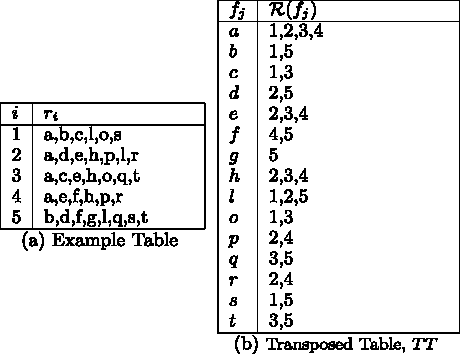
\includegraphics[width=0.5\textwidth]{res/fig/sec-3/DatasetAndTT.pdf}
  \caption{Esempio di tabella originale (a) e tabella trasposta (b), Fonte:~\cite{pan2003carpenter}}%
  \label{fig:chap-3:carpenter-tt}
\end{figure}

A differenza dei classici algoritmi di itemset mining, che esplorano lo spazio di ricerca tramite un enumerazione degli attributi, Carpenter esegue la ricerca sulla base di un enumerazione delle righe.
Questo approccio, nel caso di dataset ad alta dimensionalità, riduce lo spazio di ricerca.
Preso come esempio il dataset in~\cref{fig:chap-3:carpenter-tt} (figura a), nella \cref{subsec:apriori} si era dimostrato come una ricerca con l'algoritmo Apriori potesse potenzialmente generare \(32768\) candidati da valutare.
Una ricerca basata su righe implica considerare tutte le possibili combinazioni di righe.
Avendo il dataset in questione \(5\) righe, il numero di itemset da valutare sarà nel caso peggiore di \(32\), di tre ordini di grandezza inferiore rispetto a quello ottenuto con Apriori.

La~\cref{fig:chap-3:carpenter-ret} mostra il row enumeration tree, contenente il set completo di tutte le possibili combinazioni tra righe.
Questo albero è costruito enumerando tutte le possibili combinazioni di righe e disponendole in modo tale che ogni elemento di livello uno contenga nel suo sotto-albero tutte le possibili combinazioni tra se stesso e tutti gli elementi aventi ID maggiore del proprio.

\begin{figure}
  \centering
  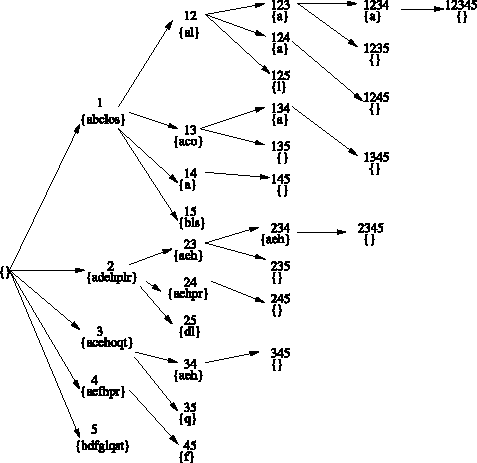
\includegraphics[width=.5\textwidth]{res/fig/sec-3/RowEnumerationTree.pdf}
  \caption{Esempio di Row Enumeration Tree, Fonte:~\cite{pan2003carpenter}}%
  \label{fig:chap-3:carpenter-ret}
\end{figure}

Per trovare i pattern chiusi e frequenti, Carpenter esegue una ricerca depth first, ovvero in cui viene stabilito un ordine lessicografico tra le transazioni e partendo da quelle avente indice più basso si esplora completamente il ramo delle possibilità collegate alla singola transazione.
Ogni elemento viene esplorato considerando solo gli elementi successivi, mai i precedenti.
In questo modo ogni possibile combinazione di righe è considerata una e una sola volta.
Ad ogni combinazione di righe è associato uno e un solo itemset chiuso, l'insieme di tutti gli itemset chiusi viene coperto considerando tutte le possibili combinazioni di righe.

Per eseguire la ricerca di itemset, poste queste condizioni, sarebbe sufficiente generare tutti le possibili combinazioni di righe, generare il loro set di attributi comuni applicando \(\mathcal{F}\) e valutare la frequenza di questo itemset.
Ciò però non sarebbe efficiente in quanto non verrebbe applicata la proprietà monotona del supporto.
Occorre quindi definire una strategia di pruning per ridurre lo spazio di ricerca.

Sia \(X\) un sottoinsieme di righe.
Data la tabella trasposta \(TT\) si definisce tabella trasposta condizionata a \(X\), denominata \(TT|_{X}\) un subset di righe di \(TT\) tale che:

\begin{enumerate}
    \item Per ogni tupla \(x\) che contiene tutti gli elementi di \(X\), esiste una tupla corrispondente in \(TT|_{X}\).
    \item Ogni tupla di \(TT|_{X}\) contiene solo elementi tali che il loro identificatore di riga è maggiore di qualunque elemento presente in \(X\).
\end{enumerate}

La \cref{fig:chap-3:carpenter-ttt} è un esempio di tabella trasposta per le transazioni \((2,3)\) del dataset in \cref{fig:chap-3:carpenter-tt}

\begin{figure}
  \centering
  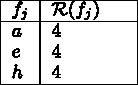
\includegraphics[width=.5\textwidth]{res/fig/sec-3/TT23.pdf}
  \caption{Tabella trasposta \(TT_{(2,3)}\) per l'insieme di transazioni \((2, 3)\), Fonte:~\cite{pan2003carpenter}}%
  \label{fig:chap-3:carpenter-ttt}
\end{figure}


Terminate le premesse, viene presentato il flusso dell'algoritmo di Carpenter (\cref{alg:carpenter}).

\begin{algorithm}[H]
\caption{Algoritmo di Carpenter}\label{alg:carpenter}
\begin{algorithmic}[1]
\Require \(F\): insieme degli attributi totali sul dataset, \(TT\): tabella trasposta, \(minsup\): soglia del supporto minimo
\Ensure \(FCP\): Pattern frequenti e chiusi

\State \(FCP \gets \varnothing\); \Comment{Inizializza l'output}
\State Dichiara R come l'insieme delle transazioni nel dataset originale ordinate per id;
\State$ MinePattern(TT|_{\varnothing}, R, FCP)$;
\State \Return \(FCP\)
\end{algorithmic}
\end{algorithm}

La logica di espansione e pruning di un itemset è contenuta all'interno del metodo \(MinePattern\) (\cref{alg:minepattern}).
In questi passi infatti viene valutata la creazione di un superset di un insieme di righe e la sua eventuale frequenza.
Durante il problema, sono definiti come \(I\) un itemset da valutare, \(X\) l'insieme delle righe che supportano \(I\) e \(R\) l'insieme delle righe da esplorare. 
Nel passo 1 dell'algoritmo viene calcolato il supporto di ogni riga \(r_i \in R\) all'interno della tabella trasposta \(TT|_X\).
A questo punto sono valutati in sequenza tre vincoli di pruning, il cui scopo è mantenere gli itemset chiusi non ancora esplorati:

\begin{enumerate}
    \item \textbf{Valutazione del superset dell'attuale set di transazioni} (passo 2).
    In questo passo viene ricercato il superset di \(X\) aggiungendo elementi di \(R\) tali che questi compaiano in almeno una riga di \(TT|_X\).
    Considerando tutti gli \(r_i,\ldots,r_n\) che soddisfano questa condizione, viene definito un superset di \(X\) \(EX = X \cup r_i \cup \ldots \cup r_n\).
    A questo punto se un superset di \(X\) non raggiunge la soglia minima di supporto, allora nessun itemset associato a una qualunque combinazione di queste righe potrà essere frequente.
    Preso come esempio il dataset in \cref{fig:chap-3:carpenter-tt} e posto \(minsup = 3\), si consideri \(X = \{3\}\) e \(R = \{4,5\}\).
    Da questo X viene generato un solo superset \(EX = \{3,4\}\), in quanto \(5\) non compare in nessuna delle transazioni di \(TT|_3\).
    Essendo \(|EX| < 3\), il processo legato all'esplorazione di questo ramo viene interrotta.
    È intuibile dalla \cref{fig:chap-3:carpenter-ret} che questo superset non potrà mai generare nessun itemset valido di \(3\) elementi.
    
    Formalmente si ricercano dentro \(R\) tutte le transazioni che compaiono in almeno una tupla di \(TT|_{X}\).
    Questo insieme viene definito come \(U\).
    Se la cardinalità di \(X \cup U\) risulta minore di \(minsup\), allora non potrà essere generato nessun itemset frequente nel superset, quindi l'esplorazione potrà essere interrotta.
    In caso contrario \(R' = U\). 
    Riferendosi all'esempio di prima \(U = {4}\), \(|X| + |U| = 2 < 3\), quindi è verificato quanto intuito sopra.
    
    \item \textbf{Eliminazione delle righe presenti in ogni tupla} (passo 3).
    Successivamente sono eliminate dall'insieme delle espansioni quelle righe che compaiono in ogni tupla della tabella trasposta \(TT|_X\).
    Questo potrebbe inizialmente sembrare un controsenso, eliminare una riga in cui \(I\) può essere espanso senza perdere elementi sembrerebbe uno sbaglio.
    Proprio per questo motivo in realtà queste righe vanno scartate.
    Scopo della creazione dei superset non è il conteggio del supporto di pattern già esistenti, quanto più l'individuare nuovi itemset non ancora valutati.
    Preso ad esempio \(X = (2,3), R = (4,5)\), \(\mathcal{F}(2,3) = \mathcal{F}(2,3,4)\) quindi la valutazione di \((2,3,4)\) non è necessaria, in quanto produrrebbe un itemset già visitato.
    
    In termini formali, le righe presenti in ogni tupla di \(TT|_X\) sono raccolte nell'insieme \(Y\), successivamente \(R' = R' - Y\).
    
    \item \textbf{Pruning degli itemset frequenti già esplorati} (passo 4).
    Ultimo passo di pruning, l'itemset che sta venendo considerato è già presente in \(FCP\), allora si può interrompere la ricerca su quel ramo.
    Intuitivamente, la natura depth-first dell'algoritmo implica che se un itemset è già presente in \(FCP\), questo sia già stato generato in un passaggio precedente dell'algoritmo.
    Questo passo di ricerca ha considerato transazioni con id inferiore a quello delle transazioni correnti, quindi sicuramente ha incluso anche quelle attualmente considerate nel calcolo del supporto.
    Ne segue che ogni possibile superset di queste righe è già stata valutata.
    Di conseguenza l'esplorazione del ramo termina.
    
    Si consideri \(X = (3, 4) \; R = (5)\) nel dataset in \cref{fig:chap-3:carpenter-tt}, \(\mathcal{F}(X) = (a,e,h)\).
    Nel momento in cui viene analizzato \(X\), \((a,e,h)\) risulta già presente in \(FCP\), in quanto generato da \(X' = (2,3), R' = (4, 5)\).
    Fissato questo, è possibile aggiungere che il superset \(EX = (3,4,5)\) risulta già valutata in \(EX' = (2,3,4,5)\).
    Questo perché se \(EX\) contenesse qualche itemset valido, questo sarebbe già individuato in \(EX'\), in quanto le righe in \(X'\) hanno id minore o uguale di quelle in X e individuano lo stesso pattern.
\end{enumerate}

Una volta che un candidato supera i tre vincoli di pruning, può essere valutato come frequente e espanso.
Nel passo 5 se l'unione tra \(X\) e \(Y\) risulta frequente, \(I\) viene aggiunto a \(FCP\), questo passaggio garantisce la validità del secondo vincolo.
Infine nel passo 6, per ogni riga in \(R'\) si esegue ricorsivamente \(MinePattern\) aggiungendo a \(X r_{i}\) e calcolando \(TT|_{X}|_{r_{i}}\)

\begin{algorithm}[H]
 \selectlanguage{italian}%
\caption{\(MinePattern(TT|_{X}, R', FCP)\)}\label{alg:minepattern}
\begin{algorithmic}[1]
\State Calcolo del supporto per ogni riga \(r_{i} \in R'\) su \(TT\). Inizializzazione di \(Y = \varnothing\); 
\State  Sia \(U \subset R'\) un set di righe che compare almeno in una tupla di \(TT_{X}\). Se \(|U| + |X| \leq minsup\) \Return altrimenti \(R' = U\). \Comment{Primo passo di pruning}
\State  Sia \(Y\) il set di righe tali che \(\forall r_{i} \in Y, r_{i} \in t_{j} \forall t_{j} \in TT|_{X}\), \(R = R - Y\) \Comment{Secondo passo di pruning}
\State  Se \(\mathcal{F}(X) \in FCP\), \Return \Comment{Terzo passo di pruning}
  \If{\(|X| + |Y| \geq minsup\)} \Comment{Se l'itemset è frequente rispetto alla soglia di supporto}
     \State \(FCP \gets \mathcal{F}(X) \cup FCP\) \Comment{La tupla viene aggiunta a FCP} 
  \EndIf
 \ForEach{\(r_{i} \in R'\)} \Comment{Per ogni elemento esplorabile}
        \State $R' = R' - {r_i}$ 
        \State $MinePattern(TT|_{X}|_{r_{i}}, R', FCP)$ \Comment{Passo ricorsivo dell'algoritmo}
    \EndFor
\end{algorithmic}
\end{algorithm}

Al termine dell'esecuzione dell'algoritmo sono riportati all'utente tutti gli itemset così individuati.


\subsection{Limiti per i dati di traiettoria}\label{subsec:cute:applicationandlimits}
Il colossal itemset mining trova diverse applicazioni nel mining di itemset.
Lo stesso algoritmo di Carpenter ha diversi utilizzi nella ricerca di dati legati al mondo della biologia o medicina.
In \cite{pan2003carpenter} vengono presentati i risultati su dataset collegati ai carcinomi a polmoni, ovaie e leucemia.
Questi risultati sono frutto del confronto tra Carpenter e altri due algoritmi di mining di itemset chiusi.
In media Carpenter risulta molto più veloce e i suoi risultati sono concordi con quanto ottenuto dagli altri due algoritmi.

Parlando poi di traiettorie, è noto che queste non sono semplici sequenze, come affermato nella \cref{subsec:fim-trajectory}.
I dati di traiettoria hanno una natura spazio-temporali che può essere utilizzata per definire tipi specifici di pattern (\cref{sec:comovement-definition}) e un pruning più efficiente.
Questo implica che i dati di traiettoria abbiano tra loro strette relazioni spazio-temporali difficili da modellare, come ad esempio vincoli di continuità temporale o contiguità spaziale.
Gli algoritmi di colossal itemset mining presenti in letteratura~\cite{DBLP:journals/bdr/ApilettiBCGPM17, DBLP:conf/kdd/PanCTYZ03} non sono pensati per sfruttare questi vincoli.
Sarebbe teoricamente possibile applicare questi vincoli a posteriori, ma sarebbe molto poco efficiente.
Questi infatti sono in grado di ridurre consistentemente lo spazio di ricerca dei possibili itemset.

Un altro problema comune negli algoritmi di colossal itemset mining è la loro natura centralizzata. 
Ad esempio Carpenter è realizzato come algoritmo centralizzato: per evitare infatti
di generare itemset già valutati in iterazione precedenti \(FCP\) viene mantenuto in un registro globale.
Tradurre questo problema in ambito distribuito pone numerose sfide.
Alcuni algoritmi in letteratura~\cite{DBLP:journals/bdr/ApilettiBCGPM17, vanahalli2019efficient} realizzano un'implementazione distribuita.

Per concludere, il colossal itemset mining è un approccio interessante per analizzare dati di traiettoria, tuttavia 
rispetto a quanto presente in letteratura si rende necessario integrare:

\begin{itemize}
    \item Dataset avente transazioni di ordini di grandezza inferiori al numero delle feature.
    \item Pruning basato su criteri spazio-temporali oltre che sulla frequenza.
    \item Gestione della continuità nel tempo e nello spazio.
    \item Implementazione distribuita.
\end{itemize}

\section{L'algoritmo CUTE}\label{sec:cute:idea}
\textit{Cu.Te}, o ClUstering TrajectoriEs, è un algoritmo di clustering overlapping il cui obbiettivo è l'analisi
di gruppi di oggetti in movimento. Questa ricerca viene condotta considerando sia la dimensione spazio-temporale
delle traiettorie sia eventuali dimensioni semantiche (come ad esempio, le municipalità di una città).

Lo scenario reale per la realizzazione di questo algoritmo è stata l'analisi condotta su
un insieme di traiettorie generate a Milano. All'interno di questo studio, i pattern di movimento sono
stati analizzati a diversi livelli.
Una prima analisi è stata condotta dividendo la superfice della città in piccole celle:questa ricerca
ha rivelato i pattern di movimento del traffico, individuando quali potessero essere le strade
maggiormente frequentate.
Succesivamente è stato realizzato uno studio basato sul vicinato: questo ha individuato i flussi di spostamento per specifiche categorie di utenti.
Infine una ricerca basata sulle municipalità ha mostrato quali fossero le aree della città più visitate da differenti gruppi di individui.

Lo scopo di \textit{Cu.Te} è dunque di estrarre i pattern di movimento che avvengono con una certa soglia di frequenza.

L'algoritmo \textit{Cu.Te} è etichettabile come algoritmo di \textit{colossal trajectory mining}.
L'idea alla base del \textit{colossal trajectory mining},
o mining di traiettorie su larga scala, interseca entrambi gli ambiti del clustering di traiettorie
e del colossal itemset mining (~\cref{subsec:problem:cim}).
La prospettiva del mining di itemset ad alta dimensionalità può essere impiegata anche nell'analisi di dati di traiettoria. Considerando la superfice
spazio-temporale coperta dall'insieme delle traiettorie e il numero di queste ultime, nella maggior parte dei casi risulterà evidente
che la dimensionalità di quest'ultimo dato sarà maggiore del precedente.
Risulta quindi possibile applicare algoritmi di mining di itemset su larga scala a dati di traiettoria.
In letteratura è possibile trovare riferimenti ad algoritmi di \textit{colossal itemset mining}~\cite{DBLP:journals/bdr/ApilettiBCGPM17, DBLP:conf/kdd/PanCTYZ03}
, tuttavia nessuno di questi è adatto alla ricerca di pattern di movimento, anche per la mancanza di
criteri di pruning basati sulle dimensioni spazio-temporali. Nonostante quindi la letteratura non
presenti una soluzione adatta, le idee alla base del \textit{colossal itemset mining} risultano sicuramente interessanti.

Parlando poi di clustering di traiettorie, rispetto a quanto trattato nella nella~\cref{sec:problem:trajectoryclustering}, è possibile aggiungere un'ulteriore divisione:
si definisce il clustering partizionante se ogni punto appartiene a un solo cluster, sovrapposto in caso contrario.
Applicando questo principio di classificazione agli algoritmi basati su traiettorie, gli algoritmi partizionanti considereranno la traiettoria nella sua interezza,
assegnandola quindi ad un solo cluster. Questa tipologia di clustering comporta però la perdita di informazioni tra i diversi cluster:
nonostante una traiettoria sia raggruppata in un cluster che massimizza la similarità tra i propri elementi,
questa può comunque condividere pattern interessanti con altre traiettorie appartenenti a cluster differenti.

Per superare il problema descritto sopra, gli algoritmi di clustering sovrapposto effettuano una divisione di ogni traiettoria
in sotto-traiettorie e effettuano un clustering partizionante su queste sotto-traiettorie.
Questa soluzione permette di conservare le relazioni intra-cluster, tuttavia una frammentazione troppo fine può causare
la perdita di \textit{rare pattern}, ad esempio eventi significanti che accadono con una bassa frequenza~\cite{DBLP:journals/tkdd/KohR16, DBLP:journals/geoinformatica/HuangPX06}.

Come già detto nella~\cref{sec:problem:trajectoryclustering}, il clustering classico non esprime vincoli temporali o ulteriori parametri adatti alla ricerca di traiettorie.
Per aggiungere la possibilità di esprimere vincoli sul tempo, sono stati introdotto i \textit{co-movement} patterns descritti nella~\cref{sec:problem:comovements-pattern}; algoritmi come \textit{G.C.M.P},
(~\cref{chapter:chapter2}), \textit{GeT Move}~\cite{DBLP:journals/ijitdm/PhanPT16} e  implementa la ricerca di questi pattern mischiando l'approccio basato su \textit{frequent itemset mining} e il clustering.
Entrambi questi framework discretizzano il tempo in bucket di dimensione finita, su cui poi applicano un clustering basato sulla densità, infine
ricercano pattern di movimento fondendo i vari cluster ottenuti nei differenti istanti temporali.

Rispetto a quanto presentato fin d'ora, \textit{Cu.Te} presenta le seguenti caratteristiche:

\begin{itemize}

  \item Flessibilità nell'impiego di dimensioni: all'interno di \textit{Cu.Te} è possibile aggiungere
  dimensioni personalizzate su cui condurre la ricerca, ad esempio si può espandere la dimensione spazio
  temporale aggiunendo il concetto di municipalità.
  Inoltre sono supportate dimensioni non esclusivamente monotone, come ad esempio i giorni della settimana.

  \item Continuità nello spazio tempo: nella ricerca di \textit{comomvement pattern} è possibile specificare vincoli di contiuità non solo sul tempo, ma anche sullo spazio.

  \item Efficienza nel pruning spazio-temporale: la strategia di pruning impiegata permette di ridurre
  lo spazio di ricerca dell'algoritmo sulla base della natura spazio-temporale delle traiettorie.

  \item Efficacia rispetto a problemi reali: \textit{Cu.Te} mette a disposizione una soluzione distribuita per il problema del \textit{Colossal Trajectory Mining}
  compatibile con dataset costruiti su problemi del mondo reale.
\end{itemize}


L'algoritmo segue tre step per la formazione dei cluster, come anche rappresentato in~\cref{fig:chap-3:cute-overview}

  \begin{figure}
    \centering
    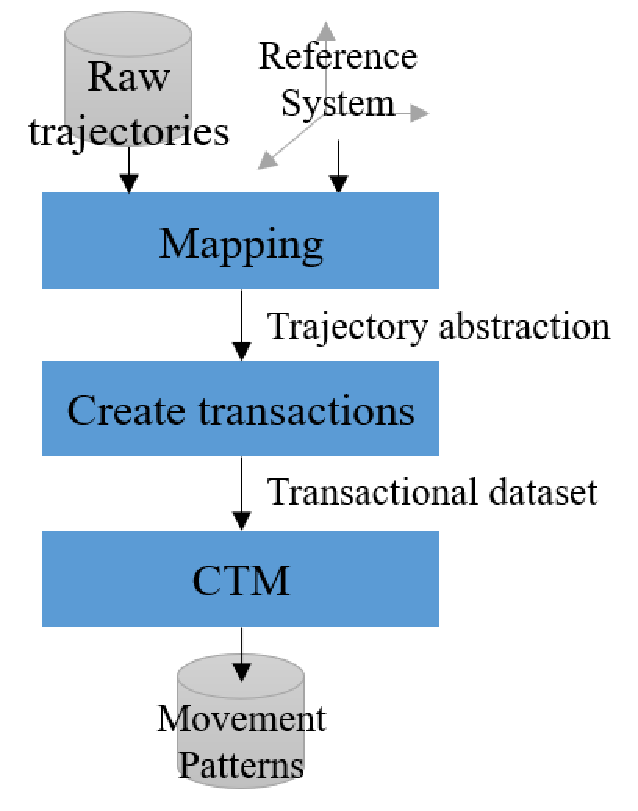
\includegraphics{/sec-3/cute-algorithm-overview.pdf}
    \caption{Rappresentazione grafica delle tre fasi dell'algoritmo Cu.Te,Fonte:~\url{https://which.souce?}}%
    \label{fig:chap-3:cute-overview}
  \end{figure}

  \begin{enumerate}
    \item \textbf{Mapping delle traiettorie:}

    In questo primo passo vengono analizzate le traiettorie presenti nel dataset. Da queste viene determinata la regione spazio-temporale
    in cui tutti gli oggetti si sono mossi. Successivamente l'area di movimento viene divisa in un insieme di celle omogenee per dimensioni nello spazio e nel tempo.
    A questo punto ad ogni traiettoria viene assegnato un insieme di celle secondo il seguente principio: una cella è attribuita ad una traiettoria quando quest'ultima ha
    almeno un punto che ricade entro i confini spazio-temporali della cella.

    \item  \textbf{Creazione delle transazioni:}

    Durante questa fase vengono poste le basi per l'\textit{itemset mining}: scopo di questa parte dell'algoritmo
    è infatti andare a generare l'insieme delle transazioni su cui verrà eseguita la ricerca di pattern.
    Ciò avviene considerando l'ouput della fase precedente e ribaltando la relazione cella traiettoria:
    mentre prima le traiettorie venivano condiderate in termini di celle percorse, ora si considera ogni cella in relazione alle traiettorie che almeno per
    un istante transitano al suo interno.

    \item \textbf{Colossal Trajectory Mining:}

    Ultima e più importante passaggio dell'algoritmo, produce in uscita i pattern di movimento.
    Dato l'output della fase precedente, ovvero un insieme di transazioni appositamemte creato,
    esegue una ricerca di itemset su dati ad alta dimensionalità.

  \end{enumerate}







\subsection{Input e parametri}\label{subsec:cute:params}
Prima di concentrarsi sui singoli passi di \textit{Cu.Te}, occorre definire la formulazione dell'algoritmo.
Innanzitutto si pone necessario riprendere i concetti di itemset, supporto e transazione descritti nella~\cref{sec:problem:frequent-itemset-mining}
e di traiettoria grezza e astrazione di traiettoria presentati nella~\cref{subsec:problem:trajectorydata}.

A queste definizioni va aggiunto il concetto di sistema di riferimento: si definisce un sistema di riferimento un insieme di
quanti completo e continuo all'interno di una regione spazio-temporale.
I sistemi di riferimento sono fondamentali nel determinare le dimensioni spazio-temporali dei punti delle varie traiettorie,
un esempio su tutti può essere una scala di riferimento espressa in coordinate polari.
Tuttavia è possibile definire anche sistemi di riferimento che utilizzano metriche diverse dalle coordinate sopracitate,
ottenendo così diversi effetti sulla rappresentazione dei dati.

Per quanto riguarda invece l'aspetto collegato alla ricerca di itemset,
in \textit{Cu.Te} viene introdotto il concetto di \textit{Cohesion} o coesione: dato un itemset \textit{I} = \{ \textit{i\textsubscript{1}},\ldots, \textit{i\textsubscript{n}}\}
avente supporto definito come \textit{s}, si definisca la funzione \textit{allTransaction(i)} %chktex 36
 che dato un item \textit{i} restituisce l'insieme delle
transazioni che lo supportano. A questo punto è possibile definire la coesione con la seguente formulazione:

\[ coh(I) = \frac{\lvert \lvert allTransaction(\textit{i\textsubscript{1}})~\cap ,\ldots, \cap~allTransaction(\textit{i\textsubscript{n}}) \rvert\rvert}{\lvert \lvert allTransaction(\textit{i\textsubscript{1}})~\cup ,\ldots, \cup~allTransaction(\textit{i\textsubscript{n}}) \rvert\rvert} \]

Considerando che il numeratore corrisponde esattamente a \textit{s}, allora è possibile esprimere l'equazione come:

\[ coh(I) = \frac{s}{\lvert \lvert allTransaction(\textit{i\textsubscript{1}})~\cup ,\ldots, \cup~allTransaction(\textit{i\textsubscript{n}}) \rvert\rvert} \]

La nuova misura permette di misurare la compattezza di un itemset rispetto agli elementi che lo compongono.
La coesione si pone quindi come meccanica di filtraggio aggiuntiva al supporto:
mentre quest'ultimo è una misura in termini assoluti di frequenza, la coesione risulta una metrica relativa alla frequenza dei singoli elementi.
Ne segue che un alto valore di coesione andrà a scartare quegli itemset i cui item risultano molto sparsi all'interno delle transazioni,
mantenendo invece quelli che risultano più compatti.

Una volta definiti questi due concetti, è opportuno elencare e definire i parametri
utilizzati da \textit{Cu.Te}.

\begin{itemize}

  \item Quanto spaziale \textit{s}:
  Definisce la dimemsione spaziale del sistema di riferimento, in relazione alle coordinate polari di ogni punto.

  \item Quanto temporale \textit{t}:
  Definisce la dimensione temporale del sistema di riferimento rispetto al tempo misurato in secondi di ogni punto di una traiettoria.
  \item Soglia di distanza spaziale\(~\epsilon \):
  Dati due punti \textit{p\textsubscript{1}, p\textsubscript{2}} e una funzione di distanza spaziale \textit{d\textsubscript{s}},
  si definisce \(~\epsilon \) come la soglia sotto la quale due punti si considerano vicini.
  \item Soglia di distanza temporale\(~\tau \): analogamente a quanto detto sopra, il parametro \(~\tau \) permette di specificare
  una soglia massima per la distanza tra due punti nel tempo.
  \item Dimensione minima\(~\gamma \): Questo parametro riguarda il numero minimo di item all'interno di ogni itemset restituito in output alla fine dell'algoritmo.
  \item Supporto minimo\(~\alpha \): La frequenza minima oltre cui ogni itemset deve apparire all'interno dell'insieme delle transazioni.
  \item Coesione minima\(~\beta \): Come definito sopra, esprime un limite inferiore alla coesione degli itemset prodotti dall'algoritmo.

\end{itemize}

Grazie a questi parametri, risulta possibile per \textit{Cu.Te} affrontare il problema
della ricerca di \textit{comovement-pattern}, descritto nella \cref{sec:problem:comovements-pattern}.
Scendendo nel dettaglio, \(~\gamma \) esprime la dimensione minima di un gruppo considerato interessante, mentre
\(~\alpha \) il numero minimo di istanti spazio-temporali in cui tutti i membri del gruppo sono considerati vicini.
\(~\epsilon \) rappresenta il criterio di vicinanza spaziale tra due punti, \(~\tau \) invece permette la ricerca dei diversi pattern di movimento:
con \(~\tau \) = 1 si ha un vincolo stringente sulla continuità temporale, andando quindi a ricercare pattern \textit{flock},
dall'altra parte con un valore uguale a \(~\infty \), si rilassa al massimo la continuità temporale, ottenendo
così dei risultati classificabili come \textit{Swarm}. Infine con qualunque valore intermedio tra 1 e  \(~\infty \),
\textit{Cu.Te} esegue la ricerca di pattern \textit{Group} degeneri, ovvero con vincolo \textit{L} posto uguale a 1.




\subsection{Mapping del dataset}\label{subsec:cute:mappingdataset}
Inizialmente, il dataset delle traiettorie è composto da un insieme di punti aventi le seguenti caratteristiche:
una dimensione temporale espressa in secondi, due coordinate spaziali per determinare la sua posizione rispetto a un sistema di coordinate polari e
infine un identificatore di traiettoria. A queste dimensioni possono essere poi aggiunte altre informazioni, che non sono prese in considerazione durante l'esecuzione dell'algoritmo.

Scopo di questa prima fase di \textit{Cu.Te} è determinare un sistema di riferimento per i punti all'interno del dataset ed esprimere questi ultimi in
relazione al nuovo sistema.

Come indicato nella~\cref{subsec:cute:parameters}, è possibile determinare un sistema di riferimento che più aderisce alle esigenze del problema.
In questo caso la necessità principale in vista della fase di \textit{Colossal Trajectory Mining} è la ridotta dimensionalità dello spazio-tempo rispetto al numero di traiettorie
processate: si rende infatti necessario avere un numero di riferimenti spazio-temporali strettamente inferiorie alle traiettorie presenti nel database.

L'idea per risolvere questa esigenza è la divisione della superficie spazio-temporale in celle omogenee per range. Dato l'intero volume dello spazio-tempo
coperto dalle traiettorie nel dataset, questo viene partizionato in parallelepipedi di medesime dimensioni. Una cella \textit{c} è un parallepipedo, generato dal
partizionamento dello spazio-tempo coperto dalle traiettorie, avente un indice univoco.
Questa suddivisione costituisce quindi il nuovo sistema di riferimento del problema, è necessario quindi esprimere i punti all'interno del dataset rispetto a questo nuovo sistema.

Partendo dallo spazio, ogni punto di traiettoria, per definizione, determina la propria posizione sulla superficie terrestre utilizzando due coordinate, latitudine e longitudine.
Prendendo in considerazione l'area di un insieme di traiettorie, il processo per la generazione di celle spaziali è il seguente: per prima cosa si determina, mediante
il parametro \textit{s} la dimensione dei lati spaziali di una cella; successivamente si definisce la funzione \textit{pointToCell}, tale funzione ha il compito
di restituire, dato un punto, la cella di appartenenza. La cella in questione viene calcolata supponendo di scomporre la superficie terrestre in quadrati aventi lato \textit{s}
a partire da Null Island (punto avente latitudine e longituidne pari a zero)~\footnote{\url{https://blogs.loc.gov/maps/2016/04/the-geographical-oddity-of-null-island/}}.
In~\cref{fig:chap-3:milan-cell-division} è possibile vedere un esempio di divisione in celle applicato sulla città di Milano.

\begin{figure}
  \centering
  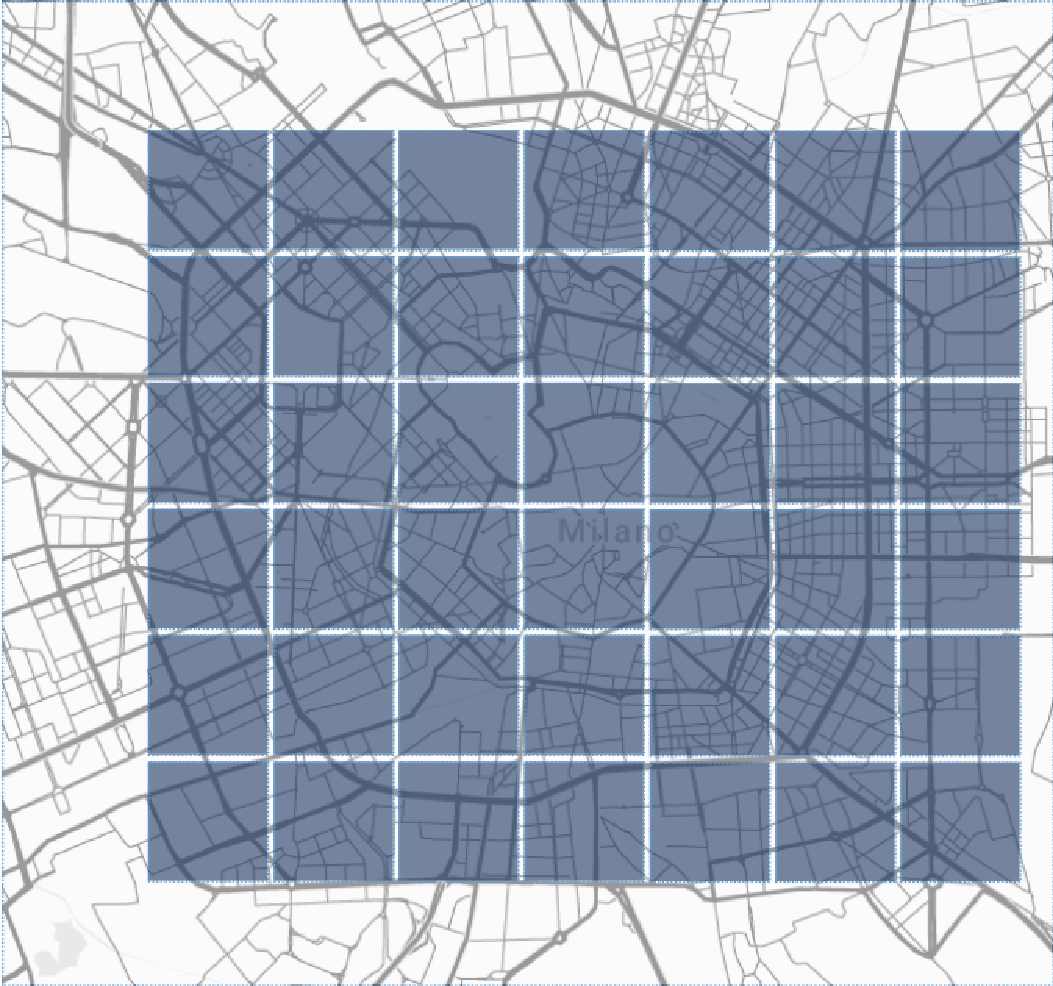
\includegraphics[scale=.6]{/sec-3/MilanCells.pdf}
  \caption{Suddivisione della città di Milano in celle,Fonte:~\url{https://which.souce?}}%
  \label{fig:chap-3:milan-cell-division}
\end{figure}

Per quanto riguarda la dimensione temporale invece, le possibilità a disposizione sono diverse, ma tra tutte si è scelto di supportare due principali scale: una basata sulle ore del giorno mentre l'altra sui giorni della settimana.
Rispetto a una metrica di tempo monotona basata su data e ora di ogni singolo punto, come ad esempio in \textit{G.C.M.P}, una scala circolare ha due vantaggi: il primo riguarda
il supporto a pattern ciclici che verrebbbero ignorati da una metrica monotona e in secondo luogo il ridotto range di valori della scala (da 0 a 23 in caso di scala giornaliera, da 0 a 6 in quella settimanale)
previene l'esplosione nel numero di celle al crescere del dataset.

Una volta determinata il lato spaziale delle celle e la durata temporale, processando le traiettorie nel dataset mediante una variazione della funzione \textit{pointToCell} adattata alla
gestione di celle tridimensionali, viene generato l'insieme delle celle \textit{C}. Questo set contiene tutte le celle, determinate dall'apposita funzione, tali che almeno
un punto di una traiettoria appartiene a quella cella. Questo approccio alla generazione delle celle garantisce che non vengano generate celle vuote, ovvero dove non passa nessuna traiettoria,
garantendo quindi una maggiore efficenza rispetto alla suddivisione assoluta della superficie spazio-temporale coperta dal dataset.

Ottenuto l'insieme delle celle, è necessario per concludere questa prima fase esprimere ogni traiettoria nel nuovo sistema di riferimento: così facendo una traiettoria non sarà più definita come
la composizione di diversi punti isolati nel tempo, ma come un'insieme di celle. La~\cref{fig:chap-3:trajectory-cell-division} mostra un esempio di conversione in un sistema di riferimento basato su celle:

\begin{figure}
  \centering
  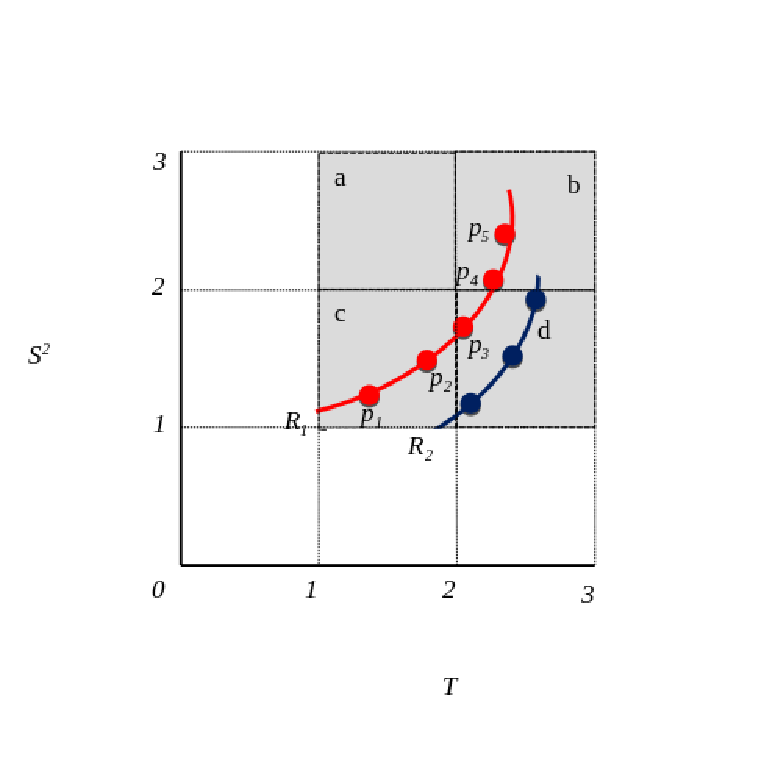
\includegraphics[scale=.8]{/sec-3/TrajectoryCellDecomposition.pdf}
  \caption{Mapping di due traiettorie, \textit{R\textsubscript{1}, R\textsubscript{2}} in un sistema di riferimento basato su celle.}%
  \label{fig:chap-3:trajectory-cell-division}
\end{figure}

Prendendo in considerazione le traiettorie \textit{R\textsubscript{1}, R\textsubscript{2}}, è possibile vedere come i punti \textit{p\textsubscript{1}, p\textsubscript{2}} appartengano alla cella \textit{c},
\textit{p\textsubscript{3}} a \textit{d} mentre \textit{p\textsubscript{4}, p\textsubscript{5}} a \textit{b}; analogamente ogni punto della traiettoria \textit{R\textsubscript{2}} sia attribuibile a \textit{d}.
Il set di celle del problema sarà quindi composto dalle seguenti celle: \textit{\textless b, c, d \textgreater} mentre le due traiettore saranno espresse in funzione del nuovo sistema di rifermimento come segue:

\begin{itemize}

  \item \textit{R\textsubscript{1}}: \{ \textit{b,c,d} \}
  \item \textit{R\textsubscript{2}}: \{ \textit{d} \}

\end{itemize}

Va sottolineato infine che, sebbene appaia nell'immagine, la cella \textit{a} non viene effettivamente generata, poiché nessuna traiettoria ha un punto entro i suoi confini.

Una volta che le traiettorie sono state espresse nelle nuove coordinate, questo primo passo dell'algoritmo giunge a termine.

Nonostante le operazioni eseguite in questa fase possano sembrare lineari, le basi che vengono gettate influenzano l'esecuzione dell'algoritmo e gli stessi risultati finali:
tra tutte, la scelta delle dimensioni di ogni cella influenza molto i passaggi successivi. Celle piccole produrranno traiettorie lunghe, estendendo il possibile spazio di ricerca di ogni cluster.
Tanto più amplio lo spazio di ricerca, tanto più a lungo dura la sua esplorazione, tuttavia è possibile eseguire una ricerca più fine su di esso.
Lati spaziali più ampli e dimensioni temporali ridotte generano celle più grandi, con uno spazio di ricerca più ridotto e risultati più grezzi.

Nonostante quanto affermato all'inizio, non è completamente corretto dire che tutti i dati che non siano collegati alla posizione nello spazio-tempo della traiettoria siano ignorati.
È infatti possibile considerare un numero variabile di dimensioni durante il processo di generazione delle celle. Tale aggiunta infatti non fa altro che andare ad aumentare la dimensionalità della singola cella,
ciò implica un numero maggiore di celle in cui dover convertire una traiettoria, ma il risultato finale della fase sarà il medesimo, l'unica differenza sarà nell'avere mediamente traiettorie
associate a un numero maggiore di celle.



\subsection{Creazione delle transazioni}\label{subsec:cute:transactioncreation}
Nella prima fase viene prodotto un dataset nella forma \textit{<t\textsubscript{i}, (c\textsubscript{1},\ldots,c\textsubscript{n})>},
dove \textit{t\textsubscript{i}} rappresenta l'id di una certa traiettoria, mentre \textit{c\textsubscript{1},\ldots,c\textsubscript{n}}
l'insieme di celle in cui tale percorso è stato convertito.
Questo dataset tuttavia non è ancora adatto ad essere sottoposto a mining, poiché in questa situazione l'insieme delle transazioni è composto dalle traiettorie,
mentre quello delle feature dalle celle.
Un'operazione di ricerca di regole associative va ad individuare tra le feature quelle che compaiono assieme con almeno una certa frequenza,
quindi in questo caso il risultato dell'algoritmo sarebbe varii raggruppamenti di celle.
Questi insiemi possono essere sicuramente utili ad individuare percorsi frequenti e trafficati, ma non sono in grado di descrivere gruppi di movimenti comuni ad un certo insieme di oggetti.

Scopo di questo secondo passo di \textit{Cu.te} è quindi modificare il dataset ottenuto dalla prima fase
in modo da renderlo valido per la ricerca di pattern di movimento.
Per realizzare questa trasformazione, occorre invertire il ruolo di celle e traiettorie all'interno del dataset: prendendo come
ipotesi di invertire la relazione tra traiettoria e insieme di celle che la compongono, si ottiene la versione trasposta del dataset originale.
La versione invertita del database sarà quindi composta dalle singole celle del problema che ora saranno identificate
come le transazioni, mentre il ruolo delle traiettorie sarà di feature. Così facendo ad ogni cella sarà associato l'insieme delle traiettorie di cui
fa parte.
In questa situazione la ricerca di itemset frequenti produce raggruppamenti di traiettorie che hanno una frequenza maggiore
a una certa soglia di supporto.
Tale soglia può essere interpretata come il numero minimo di celle, ovvero di istanti spazio-temporali, che
l'intero gruppo di traiettorie deve aver condivisio per essere considerato interessante.
Alla luce di questa interpreatzione, diviene chiaro che questo vincolo svolge la stessa identica funzione del parametro \textit{k} definito nella~\cref{sec:comovements-pattern},
per quanto riguarda invece \textit{m}, questo è espresso con  \(~\gamma \), presentato nella~\cref{subsec:cute:parameters}; infine \textit{g} è espresso come \(~\tau \) nella formalizzazione di \textit{Cu.Te}.

Invertendo il dataset è quindi possibile eseguire una ricerca di comovements pattern, ma l'inversione ha un'altra importante proprietà:
analizzando il rapporto tra il numero di celle generate nella prima fase e di traiettorie in tutto il dataset, è corretto affermare che
la quantità di queste ultime superi di gran lunga l'altra. La ricerca di pattern di movimento in città presenta infatti un'area spazio-temporale
ridotta rispetto agli oggetti che si muovono sopra questa superficie.
Di conseguenza il dataset che considera come transazioni le celle e come feature le traiettorie sarà etichettabile come dataset ad alta dimensionalità, adatto quindi a essere processato con le tecniche proprie del
\textit{Colossal Trajectory Mining}.




\subsection{Ricerca di gruppi di movimento}\label{subsec:cute:ctm}
Ultimo e più importante passaggio dell'algoritmo: dato il dataset prodotto in output dalla fase precedente,
viene eseguita una ricerca di pattern di co-movimento utilizzando i principi del \textit{Colossal Trajectory Mining}.




\subsection{Dettagli implementativi}\label{subsec:cute:implementation}
In questa sezione si tratterà di come i passaggi precedenti dell'algoritmo sono implementati e delle problematiche connesse.

Il principale problema da affrontare durante l'implementazione è stata la necessità di progettare strutture adatta a una computazione su Spark.
Rispetto a quanto visto in Carpenter occorre dunque mettere in campo strategie particolari per adattare l'algoritmo a una piattaforma distribuita.

La fase di Mapping di traiettorie (\cref{subsec:cute:mappingdataset}) viene eseguita per lo più utilizzando query SQL per determinare le varie tabelle.
In primo luogo si determina la tabella delle celle, successivamente viene effettuato un join tra quest'ultima e la tabella delle traiettorie originali.
Questa operazione ha il fine di assegnare a ogni traiettoria l'insieme delle sue celle.
Ultima tabella di supporto generata è quella del vicinato.
Il vicinato viene generato eseguendo un self join all'interno della tabella delle celle, calcolando per ogni coppia di celle la loro distanza spaziale, temporale e tra le varie dimensioni.
Tutte queste operazioni sono eseguite con Spark-SQL.
Terminata la costruzione delle tabelle accessorie, vengono create la tabella delle transazioni e quella trasposta.
Queste tabelle sono salvate come RDD e trasmesse in broadcast ai vari executors, in modo da avere sempre disponibile l'accesso a queste tabelle nelle varie fasi della computazione distribuita.

Nella fase di astrazione delle traiettorie, (\cref{subsec:cute:transactioncreation}) l'RDD contenente le coppie cella-traiettoria viene trasformato in modo da apparire nella forma cella-lista di traiettorie.
Questa operazione viene gestita con le primitive di Spark e non comporta accorgimenti particolari.

La fase di mining di gruppi (\cref{subsec:cute:ctm}) è infine la più complicata e delicata.
L'RDD cella-traiettorie della fase precedente viene trasformato nel primo livello di ricerca dell'algoritmo di Carpenter.
L'RDD così trasformato si compone di tuple nella forma: \(I, extend, X, R\).
Per esprimere i set \(I, X, R\) e in generale tutti i set contenenti transazioni o attribuiti si utilizza la classe \texttt{RoaringBitMap} (\cite{GitHubRo61:online}).
Una RoaringBitMap è un set di \(n\) bit che riesce a esprimere un set di \(n\) numeri interi.
Questa implementazione risulta efficace e efficiente, poiché permette di rappresentare i set dell'algoritmo in maniera efficiente e efficace nelle operazioni.

Trattando infine dei risultati, l'algoritmo si comporta in maniera diversa a seconda della configurazione specificata dall'utente.
I gruppi possono essere restituiti a video e salvati su tabella nel caso il loro numero diventi troppo grande per essere processati in maniera efficace.
In questo caso ad ogni passo dell'algoritmo i risultati sono processati, elaborati e poi scartati.
Nel caso invece si necessiti di avere i gruppi in una struttura dati per eseguire ulteriori calcoli, allora il processo cambia.
Tramite il flag \(toStore\) viene valutato se una tupla è già valida per essere restituita in output oppure no.
A differenza di quanto accade nel caso precedente, i gruppi validi non vengono elaborati ad ogni ciclo, ma vengono collezionati alla fine dell'esecuzione.
Per eseguire quest'operazione senza intaccare la struttura dell'algoritmo, le tuple valide vengono etichettate con il flag \(toStore\) come vero.
In questo modo possono rimanere nell'RDD senza essere processate in ulteriori operazioni, se non un ultima fase di filtraggio che elimina tutti i gruppi non validi.

\subsection{Pruning}\label{subsec:cute:pruning}
Una delle principali sfide nel distribuire l'algoritmo di Carpenter è la traduzione dei tre vincoli di pruning, pensati per funzionare in maniera centralizzata.
I primi due sono facilmente riproducibili, ma il terzo è più complicato.
La ragione è che prevede una struttura di memoria centralizzata dove inserire di volta in volta gli itemset valutati.
Ovviamente questo non è realizzabile facilmente in contesto distribuito, in quanto l'accesso in scrittura a risorse centralizzate pone diversi problemi, come ad esempio le corse critiche.
Occorre quindi formulare una nuova definizione per individuare quando un itemset sia già stato valutato o meno.
Intuitivamente, il supporto di un itemset può essere interpretato come un percorso di quanti.
Scopo della ricerca di itemset chiusi è di trovare gli itemset aventi maggior supporto: alla luce di quanto detto sopra, il supporto più grande corrisponde al percorso più lungo.
Avendo le celle un identificatore ordinato, ogni supporto può essere interpretato come un percorso che parte dal quanto con id minore e arriva in quello con supporto maggiore.
Alla luce di ciò, terzo criterio di pruning di Carpenter può essere riformulato come: ``una tupla deve essere mantenuta se questa sta costruendo il percorso più lungo per un certo itemset, altrimenti questa deve essere scartata''.

Analizzando questo nuovo criterio, il vincolo può essere descritto nei seguenti punti: 
\begin{itemize}
    \item Non devono esistere celle con ID minore all'inizio della sequenza che contengono quest'ultima nel loro vicinato.
    Intuitivamente se ciò accadesse, vorrebbe dire che il percorso massimo non comincia dall'attuale prima cella.
    In tal caso infatti esisterebbe un'altra cella che genererà lo stesso percorso che sta venendo considerato ma con supporto totale maggiore.
    Per evitare una ripetizione è necessario quindi scartare l'attuale tupla.
    \item La somma del supporto totale e delle potenziali celle che contengono l'itemset \(I\) deve avere valore maggiore di \(\alpha\).
    Se ciò non fosse vero, \(I\) non potrebbe mai raggiungere la soglia di supporto per essere considerato frequente, di conseguenza 
    sarebbe inutile espandere la tupla nelle iterazioni successive.
    \item La somma del supporto totale, delle potenziali celle che contengono l'itemset \(I\) da esplorare e delle celle antecedenti alla testa della sequenza valide per il supporto devono coprire tutte le celle che supportano \(I\).
    In caso contrario, non sarebbero mai considerate potenziali celle per l'espansione.
    
\end{itemize}
La funzione di filtraggio viene formalizzata nell'~\cref{alg:filter}
\begin{algorithm}[H]
\caption{Filter}\label{alg:filter}
\begin{algorithmic}[1]
\Require $\mathcal{T}$: Insieme delle transazioni, $N$: Vicinato, $\alpha$: soglia di supporto, $\gamma$: soglia di cardinalità.
\Ensure $l$ è frequente e potenzialmente chiuso. 
\If{$l.lcluster.size >= \gamma \wedge l.X.size + l.R.size >= \alpha$} \Comment{La tupla ha una cardinalità valida e un supporto potenzialmente buono}
\State $totalSupport = sup(l.lcluster)$ 
\If{$!N.isEmpty$}                                    \Comment{Se il vicinato è definito, la tupla deve risultare valida rispetto ai vincoli spazio-temporali}
\State $minCellID = l.X.min$
\State $OutlierCells \gets \varnothing$
\ForEach{$ cell \in totalSupport$}
\If{$cell.ID >= min.ID \vee minCellID \notin neighborhood(cell)$}
\State $OutlierCells \cup cell$
\EndIf
\EndFor
\If{$(totalSupport \setminus l.X \setminus l.R \setminus OutlierCells) == \varnothing$} \Comment{Controlla che tutte le celle continue siano dentro X o R}
\State \Return true
\EndIf
\Else  \Comment{Altrimenti controlla che X + R contenga tutte le celle che supportano \(I\)}
\If{$min(totalSupport) \in l.X \wedge (totalSupport \setminus l.X \setminus l.R) == \varnothing $}
\State \Return true
\EndIf
\EndIf
\EndIf
\State \Return false
\end{algorithmic}
\end{algorithm}

I vincoli sopra espressi permettono quindi di esprimere un filtro analogo a quello espresso nell'algoritmo di Carpenter.



